\section{Инфологическая модель}\label{sec:infological-model}

\subsection{Информационные объекты}\label{subsec:information-objects}

Выделим следующие информационные объекты:
\begin{enumerate}
    \item \textbf{Телефонный номер} \\
    Телефонный номер -- это уникальный идентификационный номер в телекоммуникационной системе связи. Этот объект характеризуется следующими атрибутами:
    \begin{enumerate}
        \item Номер:
        \begin{itemize}
            \item является уникальным идентификационным номером в телекоммуникационной системе связи;
            \item получает оператор сотовой связи;
            \item тип -- целочисленный, интервал возможных значений -- $[70000000000; 79999999999]$;
            \item используется как идентификационный номер в телекоммуникационной системе связи;
            \item администратор и абонент не имеют никакого доступа, продавец-консультант имеет только доступ для чтения.
        \end{itemize}

        \item Свободность:
        \begin{itemize}
            \item является обозначением <<занят>> или <<свободен>> телефонный номер;
            \item определяется как <<занят>>, если существует абонент, на которого зарегистрирован данный телефонный номер, иначе -- <<свободен>>;
            \item тип -- бит, 0 -- <<занят>>, 1 -- <<свободен>>;
            \item используются для поиска свободных номеров;
            \item администратор и абонент не имеют никакого доступа, продавец-консультант имеет доступ для чтения и записи.
        \end{itemize}
    \end{enumerate}
    \begin{figure}[H]
        \label{fig:telephone-number-attributes}
        \caption{Взаимосвязи атрибутов объекта <<Телефонный номер>>}
        \center{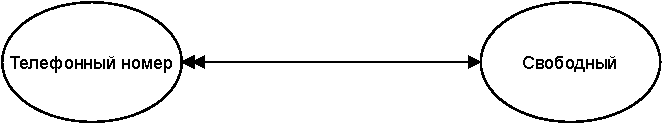
\includegraphics{graphics/telephone-number-attributes}}
    \end{figure}

    \item \textbf{Тариф} \\
    Тариф -- это включаемые услуги и ставки оплаты за эти же услуги, предоставляемые компанией. Этот объект характеризуется следующими атрибутами:
    \begin{enumerate}
        \item Название:
        \begin{itemize}
            \item является уникальным идентификатором тарифа;
            \item разрабатывается менеджером (или группой менеджеров) компании сотового оператора;
            \item тип -- текстовый, максимальный размер -- 64 символа;
            \item используется как обозначение тарифа;
            \item администратор имеет доступ для чтения и записи, продавец-консультант и абонент имеют только доступ для чтения.
        \end{itemize}

        \item Абонентская плата:
        \begin{itemize}
            \item является размером платы за тариф;
            \item разрабатывается менеджером (или группой менеджеров) компании сотового оператора;
            \item тип -- числовой, интервал возможных значений -- $[150; 5000]$;
            \item используется как описание размера платы за тариф;
            \item администратор имеет доступ для чтения и записи, продавец-консультант и абонент имеют только доступ для чтения.
        \end{itemize}

        \item Интернет трафик:
        \begin{itemize}
            \item является размером предоставляемой компанией соответствующей услуги;
            \item разрабатывается менеджером (или группой менеджеров) компании сотового оператора;
            \item тип -- числовой, интервал возможных значений -- $[0; \infty]$; % или же обозначить бесконечность как -1
            \item используется как описание размера предоставляемой компанией соответствующей услуги;
            \item администратор имеет доступ для чтения и записи, продавец-консультант и абонент имеют только доступ для чтения.
        \end{itemize}

        \item Количество минут:
        \begin{itemize}
            \item является размером предоставляемой компанией соответствующей услуги;
            \item разрабатывается менеджером (или группой менеджеров) компании сотового оператора;
            \item тип -- целочисленный, интервал возможных значений -- $[0; \infty]$; % или же обозначить бесконечность как -1
            \item используется как описание размера предоставляемой компанией соответствующей услуги;
            \item администратор имеет доступ для чтения и записи, продавец-консультант и абонент имеют только доступ для чтения.
        \end{itemize}

        \item Количество SMS:
        \begin{itemize}
            \item является размером предоставляемой компанией соответствующей услуги;
            \item разрабатывается менеджером (или группой менеджеров) компании сотового оператора;
            \item тип -- целочисленный, интервал возможных значений -- $[0; \infty]$; % или же обозначить бесконечность как -1
            \item используется как описание размера предоставляемой компанией соответствующей услуги;
            \item администратор имеет доступ для чтения и записи, продавец-консультант и абонент имеют только доступ для чтения.
        \end{itemize}
    \end{enumerate}
    \begin{figure}[H]
        \label{fig:tariff-attributes}
        \caption{Взаимосвязи атрибутов объекта <<Тариф>>}
        \center{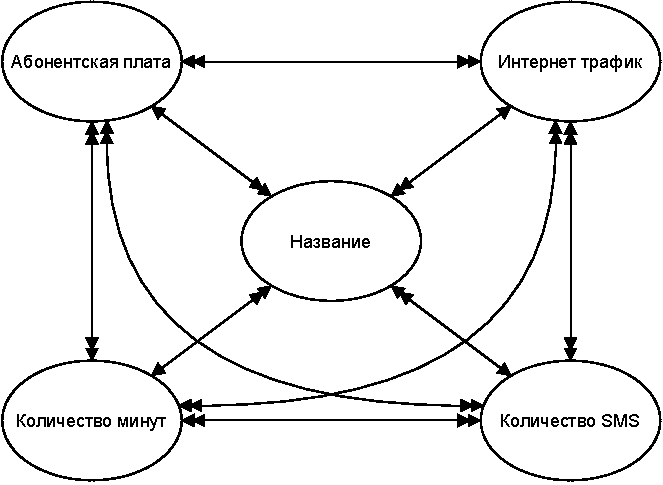
\includegraphics{graphics/tariff-attributes}}
    \end{figure}

    \item \textbf{SIM-карта} \\
    SIM-карта -- это идентификационный электронный модуль мобильной связи сотового оператора. Этот объект характеризуется следующими атрибутами:
    \begin{enumerate}
        \item Расчётный счёт:
        \begin{itemize}
            \item является номером банковского счёта и уникальным номером идентификатором SIM-карты;
            \item выдаётся банком, с которым компания сотового оператора состоит в партнёрских отношениях;
            \item тип -- целочисленный, интервал возможных значений -- $[10000000000000000000; 99999999999999999999]$;
            \item используется как номер банковского счёта для оплаты за услуги;
            \item администратор не имеет никакого доступа, продавец-консультант и абонент имеют только доступ для чтения.
        \end{itemize}

        \item Телефонный номер:
        \begin{itemize}
            \item является идентификационным номером, зарегистрированным на данную SIM-карту, в телекоммуникационной системе связи;
            \item регистрируется на SIM-карту с заключением договора;
            \item тип -- целочисленный или null, интервал возможных значений -- $[70000000000; 79999999999]$;
            \item используется как идентификационный номер в телекоммуникационной системе связи;
            \item администратор не имеет никакого доступа, продавец-консультант имеет доступ для чтения и записи, абонент имеет только доступ для чтения.
        \end{itemize}

        \item Подключённый тариф:
        \begin{itemize}
            \item является названием тарифа, зарегистрированного на данную SIM-карту;
            \item регистрируется на SIM-карту с заключением договора;
            \item тип -- текстовый или null, максимальный размер -- 64 символа;
            \item используется для определения зарегистрированного тарифа на данную SIM-карту;
            \item администратор не имеет никакого доступа, продавец-консультант имеет только доступ для чтения, абонент имеет доступ для чтения и записи.
        \end{itemize}
    \end{enumerate}
    \begin{figure}[H]
        \label{fig:sim-card-attributes}
        \caption{Взаимосвязи атрибутов объекта <<SIM-карта>>}
        \center{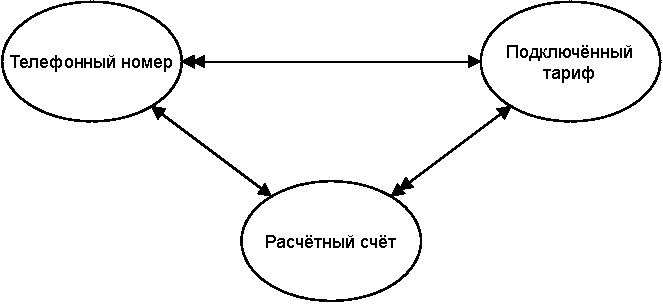
\includegraphics{graphics/sim-card-attributes}}
    \end{figure}

    \item \textbf{Клиент} \\
    Клиент -- это лицо, заинтересованное в получении услуг данной компании. Клиент характеризуется следующими атрибутами:
    \begin{enumerate}
        \item Номер паспорта:
        \begin{itemize}
            \item является идентификационным номером документа клиента, подтверждающего его личность;
            \item берётся из паспорта клиента;
            \item тип -- целочисленный, интервал возможных значений -- $[0100000101; 9999999999]$;
            \item используется как идентификационный номер клиента в системе;
            \item администратор не имеет никакого доступа, продавец-консультант имеет доступ для чтения и записи, абонент имеет только доступ для чтения.
        \end{itemize}

        \item Фамилия:
        \begin{itemize}
            \item является частью имени, по которому обращаются к клиенту;
            \item берётся из паспорта клиента;
            \item тип -- строковый, максимальный размер -- 64 символа;
            \item используется как часть имени, по которому обращаются к клиенту;
            \item администратор не имеет никакого доступа, продавец-консультант имеет доступ для чтения и записи, абонент имеет только доступ для чтения.
        \end{itemize}

        \item Имя:
        \begin{itemize}
            \item является частью имени, по которому обращаются к клиенту;
            \item берётся из паспорта клиента;
            \item тип -- строковый, максимальный размер -- 64 символа;
            \item используется как часть имени, по которому обращаются к клиенту;
            \item администратор не имеет никакого доступа, продавец-консультант имеет доступ для чтения и записи, абонент имеет только доступ для чтения.
        \end{itemize}

        \item Отчество:
        \begin{itemize}
            \item является частью имени, по которому обращаются к клиенту;
            \item берётся из паспорта клиента;
            \item тип -- строковый или null, максимальный размер -- 64 символа;
            \item используется как часть имени (если имеется), по которому обращаются к клиенту;
            \item администратор не имеет никакого доступа, продавец-консультант имеет доступ для чтения и записи, абонент имеет только доступ для чтения.
        \end{itemize}

        \item Место прописки:
        \begin{itemize}
            \item является названием места, по которому прописан клиент;
            \item берётся из паспорта клиента;
            \item тип -- строковый, максимальный размер -- 256 символа;
            \item используется как служебная информация о клиенте;
            \item администратор не имеет никакого доступа, продавец-консультант имеет доступ для чтения и записи, абонент имеет только доступ для чтения.
        \end{itemize}
    \end{enumerate}
    \begin{figure}[H]
        \label{fig:client-attributes}
        \caption{Взаимосвязи атрибутов объекта <<Клиент>>}
        \center{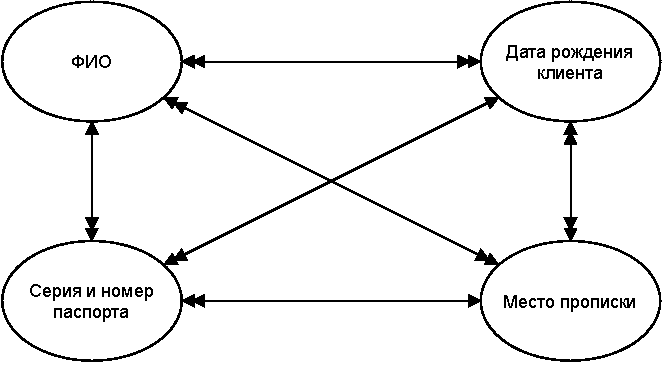
\includegraphics{graphics/client-attributes}}
    \end{figure}

    \item \textbf{Абонент} \\
    Абонент -- это пользователь услугами сотового оператора. Абонент характеризуется следующими атрибутами:
    \begin{enumerate}
        \item Телефонный номер:
        \begin{itemize}
            \item является уникальным идентификационным номером абонента в телекоммуникационной системе связи;
            \item выдаётся абоненту с заключением договора;
            \item тип -- целочисленный, интервал возможных значений -- $[70000000000; 79999999999]$;
            \item используется как идентификационный номер абонента в телекоммуникационной системе связи;
            \item администратор не имеет никакого доступа, продавец-консультант имеет доступ для чтения и записи, абонент имеет только доступ для чтения.
        \end{itemize}

        \item Абонентский счёт:
        \begin{itemize}
            \item является номером банковского счёта абонента;
            \item выдаётся абоненту с заключением договора;
            \item тип -- целочисленный, интервал возможных значений -- $[10000000000000000000; 99999999999999999999]$;
            \item используется как номер банковского счёта абонента для оплаты за услуги;
            \item администратор не имеет никакого доступа, продавец-консультант имеет доступ для чтения и записи, абонент имеет только доступ для чтения.
        \end{itemize}

        \item Номер паспорта:
        \begin{itemize}
            \item является идентификационным номером документа абонента, подтверждающего его личность;
            \item берётся из паспорта абонента;
            \item тип -- целочисленный, интервал возможных значений -- $[0100000101; 9999999999]$;
            \item используется как идентификационный номер абонента в системе;
            \item администратор не имеет никакого доступа, продавец-консультант имеет доступ для чтения и записи, абонент имеет только доступ для чтения.
        \end{itemize}

        \item Фамилия:
        \begin{itemize}
            \item является частью имени, по которому обращаются к абоненту;
            \item берётся из паспорта абонента;
            \item тип -- строковый, максимальный размер -- 64 символа;
            \item используется как часть имени, по которому обращаются к абоненту;
            \item администратор не имеет никакого доступа, продавец-консультант имеет доступ для чтения и записи, абонент имеет только доступ для чтения.
        \end{itemize}

        \item Имя:
        \begin{itemize}
            \item является частью имени, по которому обращаются к абоненту;
            \item берётся из паспорта абоненту;
            \item тип -- строковый, максимальный размер -- 64 символа;
            \item используется как часть имени, по которому обращаются к абоненту;
            \item администратор не имеет никакого доступа, продавец-консультант имеет доступ для чтения и записи, абонент имеет только доступ для чтения.
        \end{itemize}

        \item Отчество:
        \begin{itemize}
            \item является частью имени, по которому обращаются к абоненту;
            \item берётся из паспорта абонента;
            \item тип -- строковый или null, максимальный размер -- 64 символа;
            \item используется как часть имени (если имеется), по которому обращаются к абоненту;
            \item администратор не имеет никакого доступа, продавец-консультант имеет доступ для чтения и записи, абонент имеет только доступ для чтения.
        \end{itemize}

        \item Место прописки:
        \begin{itemize}
            \item является названием места, по которому прописан абонент;
            \item берётся из паспорта абонента;
            \item тип -- строковый, максимальный размер -- 256 символа;
            \item используется как служебная информация о абоненте;
            \item администратор не имеет никакого доступа, продавец-консультант имеет доступ для чтения и записи, абонент имеет только доступ для чтения.
        \end{itemize}
    \end{enumerate}
    \begin{figure}[H]
        \label{fig:subscriber-attributes}
        \caption{Взаимосвязи атрибутов объекта <<Абонент>>}
        \center{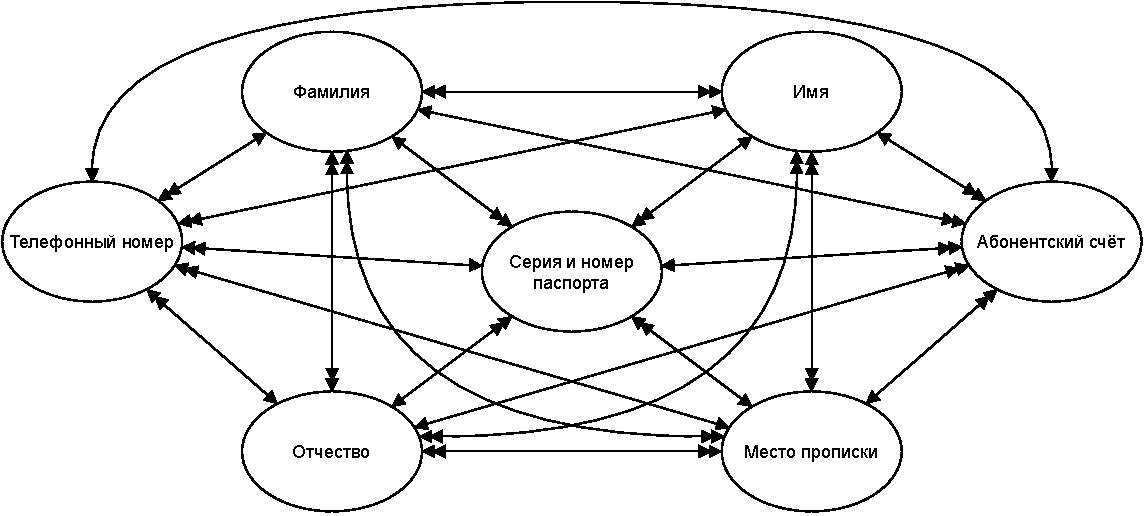
\includegraphics[scale=0.75]{graphics/subscriber-attributes}}
    \end{figure}
\end{enumerate}